\ifx\mlbook\undefined
    \providecommand{\pathroot}{../../..}

    \title{Deep Belief Network}
    \author{Donald Cheung\\jianzhang9102@gmail.com}
    \date{\today\footnote{文档编写开始于2018年2月1日}}

    \documentclass[a4paper,10pt]{ctexbook}
\usepackage{xeCJK}
\usepackage{fontspec}
\usepackage{minted}
\usepackage[CJKbookmarks,colorlinks,linkcolor=red]{hyperref}
\usepackage{geometry}
\usepackage{amsmath}
\usepackage[format=hang,font=small,textfont=it]{caption}
\usepackage{float}
\usepackage{subfigure}
\usepackage[nottoc]{tocbibind}
\usepackage{bm}

\setmainfont{Times New Roman}
\setsansfont{Helvetica}
\setmonofont{Courier New}
\setCJKmainfont[BoldFont={SimHei},ItalicFont={SimHei}]{SimSun}
\setCJKsansfont{SimSun}
\setCJKmonofont{SimSun}

\geometry{left=3.0cm,right=3.0cm,top=2.5cm,bottom=2.5cm}

\newenvironment{myquote}{\begin{quote}\kaishu\zihao{-5}}{\end{quote}}
\newcommand\degree{^\circ}
\newtheorem{thm}{定理}

\bibliographystyle{plain}

\begin{document}
\maketitle
\tableofcontents

\fi

\chapter{Deep Belief Network}


文献 \cite{hinton2006fast} 总体描述了DBN算法的实现。
我认为DBN算法就是Wake-Sleep算法+RBM,文中讨论了Explaining away,complementary prior两个重要概念。讨论了RBM与Infinite directed model with tied weights的等价性。

但是论文对Wake-Sleep算法解释特别少,因此,我对为什么讨论Explaining away,complementary prior两个概念非常不理解,云里雾里。使得我对为什么要用Wake-Sleep算法+RBM来学习多层神经网络非常难以理解。


文献 \cite{hinton1995wake} 研究了Wake-Sleep算法。

多层神经网络有很好的特征表达能力,但许多学习算法效率不高。
Wake-Sleep算法是一种有效的多层神经网络学习算法。

它使得训练数据的表示最经济,同时能够准确地重构训练数据。
训练数据的表示分布(representation)记为 $Q(\alpha | d)$,训练数据的生成分布(generation)记为 $P(\alpha|d)$。
学习的目标是:使得描述长度(description length)最小。即:
\[
    C(d) = \sum_{\alpha} Q(\alpha | d) C(\alpha, d) − (−\sum_{\alpha}(Q(\alpha | d) \log Q(\alpha | d)))
\]

在Wake阶段使得 $P(\alpha|d)$ 逼近 $Q(\alpha|d)$,在Sleep阶段使得 $Q(\alpha | d)$ 逼近 $P(\alpha | d)$。
但是,由于 $Q(\alpha | d)$ 为因子形式分布(factorial distribution),很难准确地匹配 $P(\alpha | d)$。
因为 $P(\alpha | d)$ 的公式为:
\[
    P(\alpha | d) = e^{−C(\alpha,d)} \sum_{\beta} e^{−C(\beta,d)}
\]
在一般情况下是不具备因子形式的分布。因此 $Q(\alpha | d)$ 难以匹配 $P(\alpha | d)$,从而加大了学习误差。
为了改善Wake-Sleep算法,需要使得似然分布 $P(d | \alpha)$ 对应的后验分布 $P(\alpha | d)$ 具有因子形式分布。
互补先验分布(Complementary Prior)就能够保证因子形式的似然分布具有因子形式的后验分布。
这点在文献 \cite{hinton2006fast} 的附录中讨论得很清楚。

RBM的作用就是用来生成似然分布的互补先验分布,使得其后验分布具有因子形式。
因此,DBN算法解决了Wake-Sleep算法表示分布难以匹配生成分布的难题,通过RBM使得训练数据的生成分布具有因子形式,从而提高了学习效率。


\section{受限玻尔兹曼机}

RBM (Restricted Bolzman Machine)

G. Hinton 提出了名为对比散度 (Contrastive Divergence,如图\ref{fig:contrastive_divergence}) 的学习算法。

\begin{figure}[ht]
    \centering
    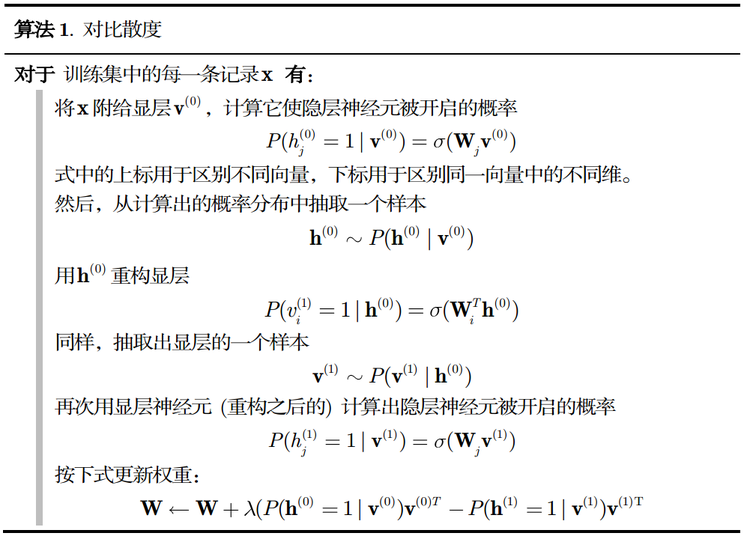
\includegraphics[scale=0.7]{\pathroot/theory/neural_networks/dbn/images/contrastive_divergence.png}
    \caption{对比散度算法}
    \label{fig:contrastive_divergence}
\end{figure}



学习材料
\begin{enumerate}
\item 1. Representation Learning: A Review and New Perspectives, Yoshua Bengio, Aaron Courville, Pascal Vincent, Arxiv, 2012.
\item 2. The monograph or review paper Learning Deep Architectures for AI (Foundations \& Trends in Machine Learning, 2009).
\item 3. Deep Machine Learning – A New Frontier in Artificial Intelligence Research – a survey paper by Itamar Arel, Derek C. Rose, and Thomas P. Karnowski.
\item 1. Introduction to Restricted Boltzmann Machines by Edwin Chen.
\item 2. An Introduction to Restricted Boltzmann Machines by Yuhuan Jiang.
\item 3. Restricted Boltzmann Machine - Short Tutorial by iMonad.
\item 4. 《深度学习学习笔记整理系列》 by Zouxy.
\end{enumerate}



\ifx\mlbook\undefined
    \bibliography{\pathroot/reference/reference.bib}
\end{document}

\fi
